Som et proof of concept er der valgt at implementere en enkelt metode til at detektere hvor vidt man sover eller ej.
Metoden der tages udgangspunkt i er den metode som er beskrevet i \cref{sec:BES} altså Best Effort Sleep, men andre metoder kunne også have været brugt.
Der vil dog kun tages udgangspunkt i de sensorer der har fået givet en høj koefficient, som kan ses i \cref{tab:vaegtninger}, hvilket gør at amplitude og acceleration er de datatyper der tages udgangspunkt i.
Disse to data typer kombineres til en enkelt model der vurderer om man sover.

\subsection{Sensor Data}
Hoved ideen bag brugen af acceleration og amplitude data kan ses i \cref{sec:BES}, men den dækker ikke alle problemscenarier der kan være involveret i brugen af disse data.

For at have en bedre indsigt i hvordan vi kan bruge accelerations og amplitude data blev disse plottet over en dag inklusiv søvn, hvor man holdt log for hvornår der blev sovet.
Dette resulterede i \cref{fig:accplot} og \cref{fig:amplplot}.

\begin{figure}[h]
	\centering
	%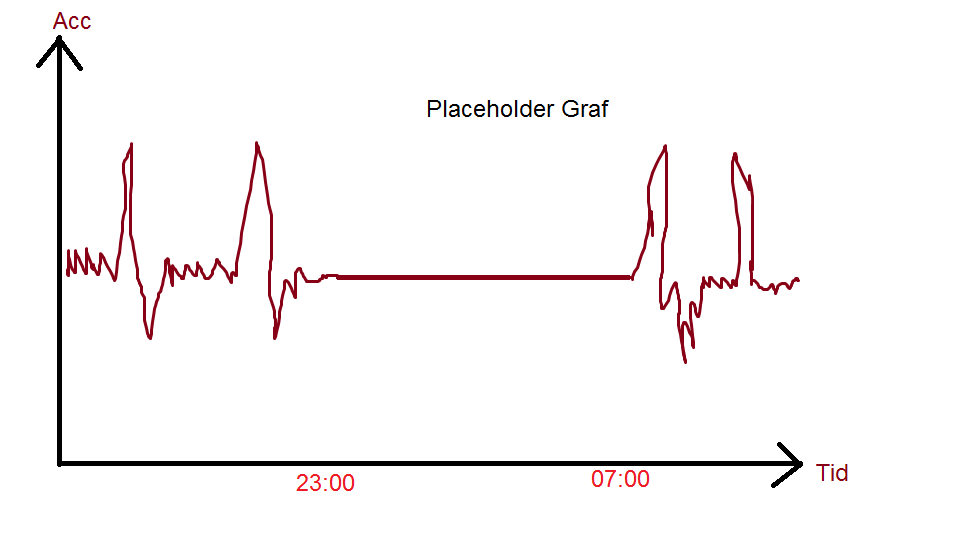
\includegraphics[scale=0.5]{acc-placeholder}
	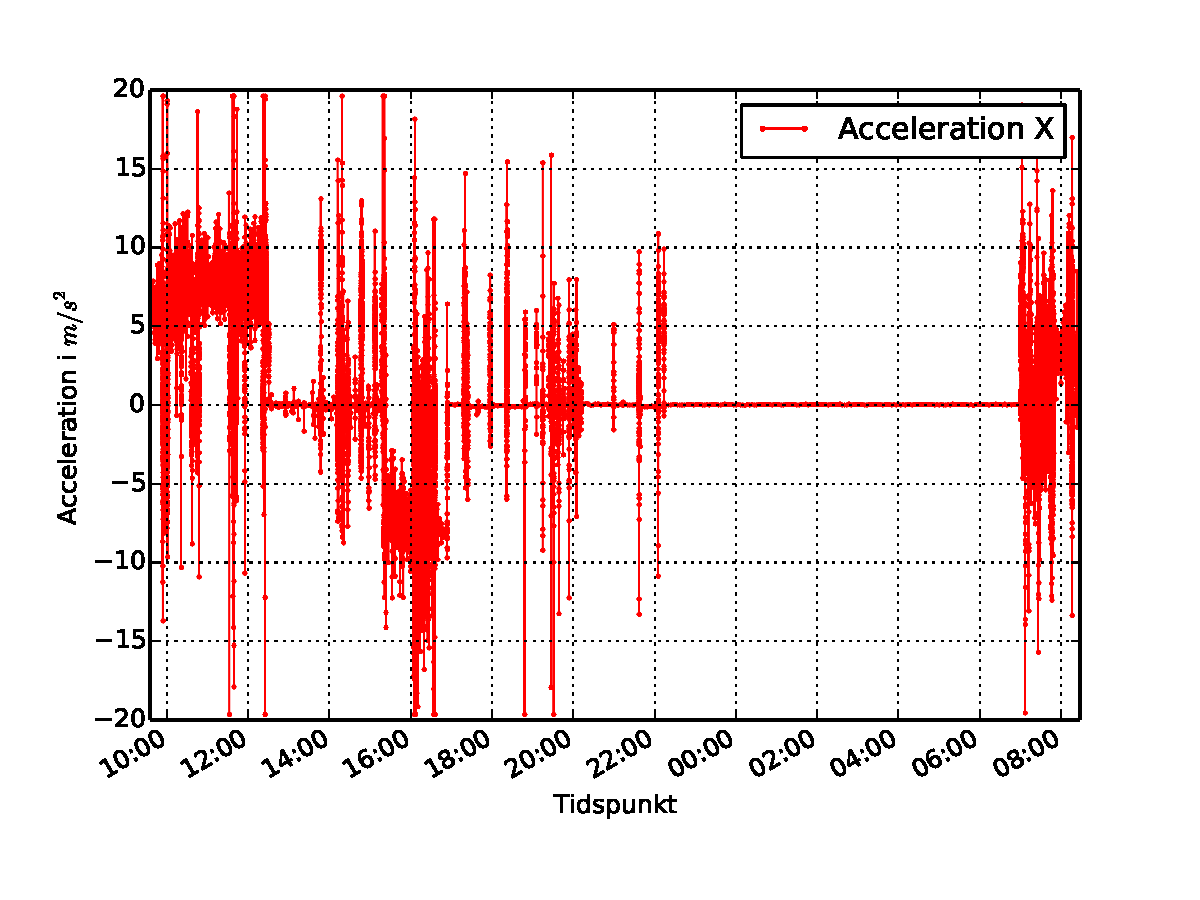
\includegraphics[scale=0.75]{acceleration-plot}
	\caption{Accelerationsplot, hvor der blev sovet fra ca. 22:00 til 07:00 næste dag.}\label{fig:accplot}
\end{figure}


Ses der på accelerometer data i \cref{fig:accplot} indikerer det tydeligt når telefonen har været i bevægelse og når telefonen ikke har været i bevægelse.
Dette skyldes at accelerometret er god til at registrere bevægelse, da acceleration er ændring i hastighed.
Det viser sig at plottet fint indikerer når man er vågen, hvilket er forårsaget af at testpersonen har gået med sin telefon i lommen.
Dog kan man ved stilstand ikke vide sig sikker på om det er fordi man sover, eller blot fordi man har lagt sin mobil fra sig.

Ved stilstand i en længere periode kan det forsøges at estimere sandsynligheden for at denne stilstand er grundet at man sover, men derudover kan andre sensor inputs hjælpe til at klargøre denne tvivl, der ikke er begrænset til at man skal have telefonen i lommen.
Et eksempel på en sådan kilde er mikrofonen, som vi kan bruge til at måle maksamplitude, således at man ikke indsamler personfølsomme oplysninger da man ikke kan genskabe en samtale men blot har maksamplitude lagret for hvert sekund.

\begin{figure}[h]
	\centering
	%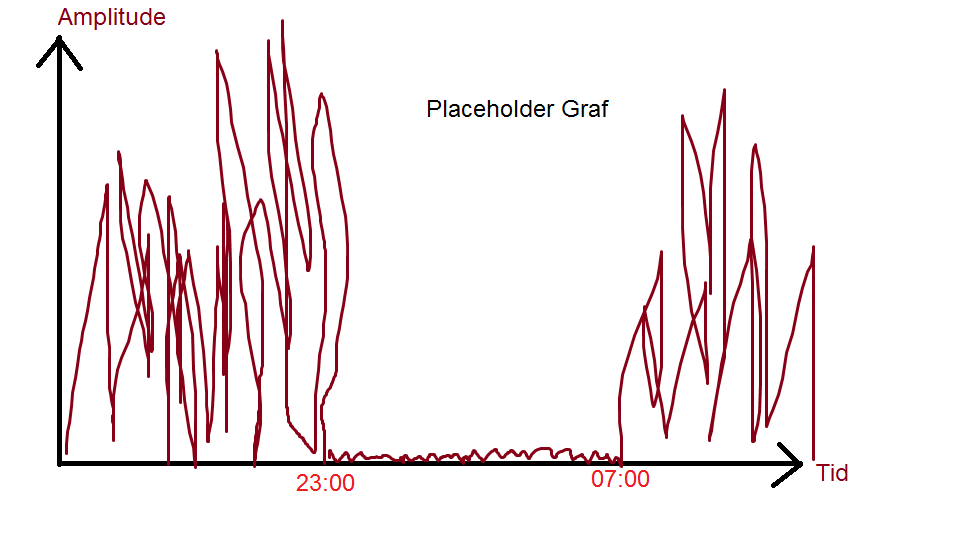
\includegraphics[scale=0.5]{ampl-placeholder}
	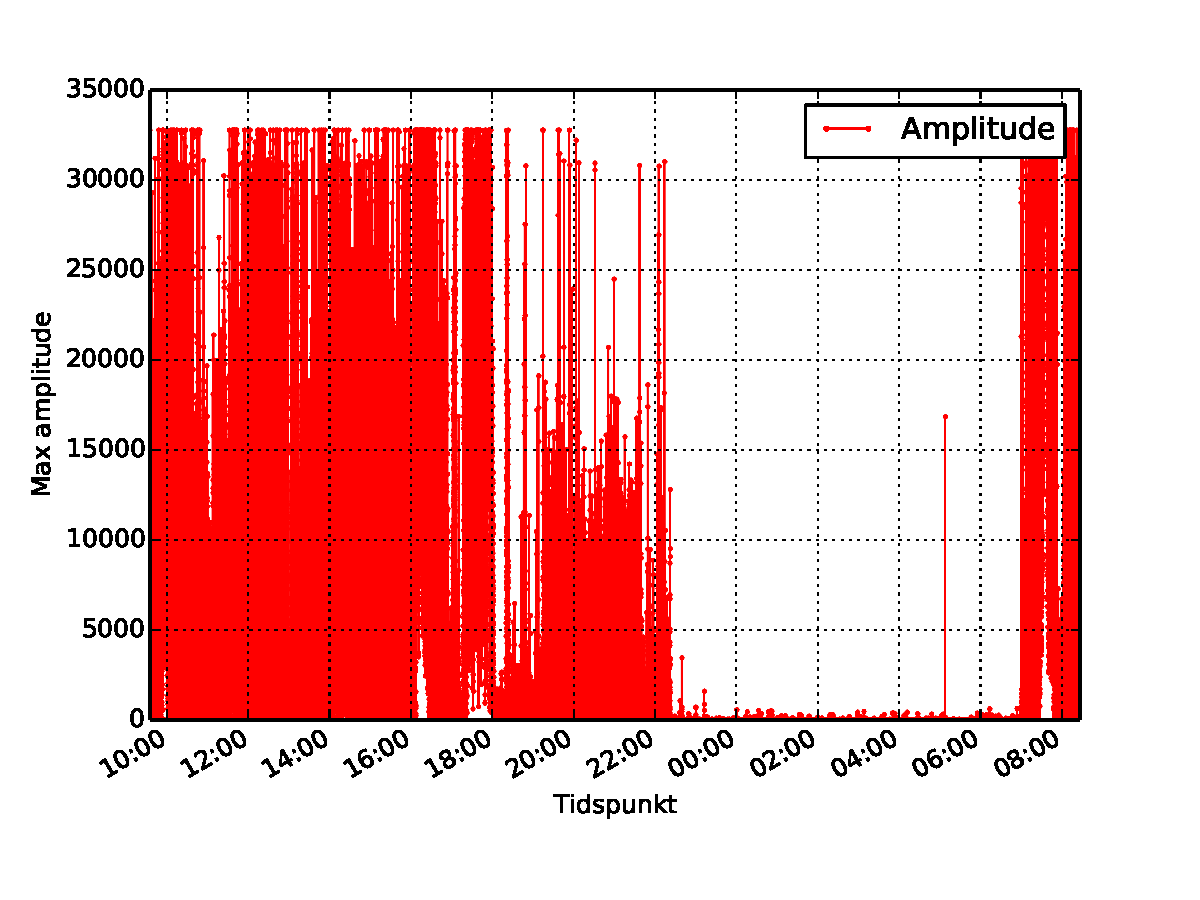
\includegraphics[scale=0.75]{amplitude-plot}
	\caption{Amplitudeplot, hvor der blev sovet fra ca. 22:00 til 07:00 næste dag.}\label{fig:amplplot}
\end{figure}

Idéen bag at bruge maksamplituden er at man larmer væsentligt mere når man er vågen end når man sover.
Dette passer fint med de loggede data plottet i \cref{fig:amplplot}.
Dog har denne antagelse også begrænsninger.
Eksempelvis kan det være at man er en stille person, snorker meget eller også kunne personen bo i et meget larmende område.
Alligevel regner vi med at amplituden stadig kan bruges, da man så muligvis kunne finde et mønster når man snorker,\als{nævn nogle algoritmer der kan gøre dette? Så kan vi referere at det helt sikkert er muligt men ikke gjort grundet begrænset tid} og muligvis begiver sig hen i støjende områder når man er vågen.
Derudover er det så et spørgsmål om hvor stor vægt man skal tillægge de enkelte sensorkilder og er noget der bør trænes til det enkelte individ for at opnå en model der passer til det enkelte individs personlighed.
Hvordan dette gøres bør overvejes ved videreudvikling, men til dette proof of concept kan man som en start bruge fastsatte statiske vægte.

\subsection{Søvnestimerings model}
Ud fra observeret data etablerer vi nogle antagelser som vi går ud fra holder til fremtidigt data også.
Disse er at når man observerer en handling om det er acceleration eller amplitude, kan vi med stor sikkerhed sige at man ikke sover.
Modsat ved stilstand er sandsynligheden for at man sover afhængigt af længden af stilstand.
Dette får os til at lave en model der bygger på disse to antagelser.

Vi kan med andre ord sige følgende:
\begin{equation}
P(t,t_0) =
\begin{cases}
0	& t = t_0 \\
min(s(t-t_0),1) & \text{ellers}
\end{cases}
\end{equation}
hvor,
\begin{itemize}
	\item[$P(t,t_0)$] Sandsynligheden for at man sover mellem $t$ og $t_0$. 
	\item[$t$] Tiden for observeret data.
	\item[$t_0$] Sidste tid med bevægelse/lyd.
\end{itemize}
Hvis vi formulerer problemet på denne måde er det et spørgsmål om at ændre $t_0$ når der observeres et væsentligt udsving i ens data, der indikerer man er vågen.
Derudover vil $t-t_0$ så svare til længden af stilstand eksempelvis målt i timer.

Spørgsmålet går så på hvorledes funktionen $s(t-t_0)$ skal defineres.
Det skal være en funktion der repræsenterer hvor sikker man er på søvn ud fra længden af stilstand eksempelvis målt i timer.
En sådan funktion bør være lært ud fra ens empiri, så man kunne løse opgaven som et regressionsproblem.
Dette er et område der kan arbejdes videre med for at få en mere akkurat søvnestimeringsmetode og opfordres til at gøre med mere tid.

Dog for at få et udgangspunkt til diskussion af sådanne funktioner er der tre funktioner plottet i \cref{fig:trefunc}.
\begin{figure}[h]
	\centering
	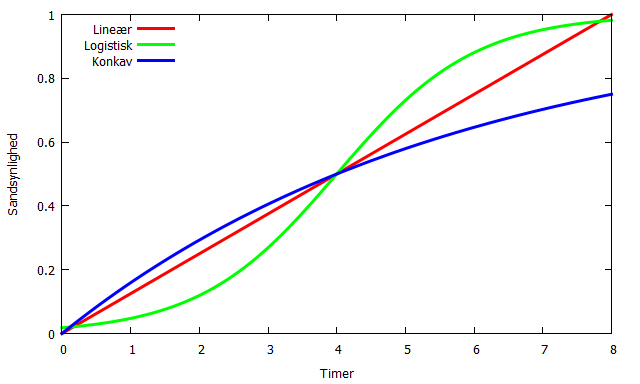
\includegraphics[scale=0.5]{graf-funktionseksempler}
	\caption{Tre funktioner til estimering af sandsynlighed for søvn}\label{fig:trefunc}
\end{figure}

\cref{fig:trefunc} viser tre forslag til funktioner for $s(t-t_0)$.
Disse er den røde lineære funktion, den blå konkave funktion og den grønne logistiske funktion.
Alle tre funktioner har til fælles at de er voksende, hvilket passer med vores antagelse af jo længere der har været stilstand jo større sandsynlighed for at man sover.
Den lineære funktion bygger på antagelsen at sandsynligheden for at man sover er kongruent med stilstands længden, hvilket vi ikke ønsker da vi så tillægger for stor vægt til korte stilstandsperioder.
Af samme grund forkastes den konkave funktion også.

Til sidst har vi den logistiske funktion der fint beskriver hvordan at ved længere stilstandsperioden er der en forøget hældning i funktionen indtil vi nærmer os lange stilstandsperioder hvor ekstra tid ikke giver megen ekstra sandsynlighed for søvn men stadig lidt, dette kan ses da den logistiske funktion vi har plottet går asymptotisk mod 1, svarende til 100\% sikkerhed for søvn.
I realiteten kan vi aldrig være 100\% sikker på søvn ved lang stilstand, det kan være man har glemt mobilen hjemme mens man er på tur over en weekend, men hvis forudsætningen for at systemet fungerer er at man har mobilen i nærheden regnes den logistiske funktion som et godt redskab til et søvnestimat.

Definitionen af $s(t-t_0)$ hvor vi kalder $t-t_0$ for $t_{span}$ er dermed følgende:
\begin{equation}
	s(t_{span}) = \frac{L}{1+e^{k*(-t_{span} - t_{midpoint})}}
\end{equation} 
hvor,
\begin{itemize}
	\item[$t_{midpoint}$] er til hvilket stilstandslængde vi vil have sandsynligheden for søvn til at være 50\%, dette kan eksempelvis være $4$ timer.
	\item[$k$] er stejlheden for kurven.
	\item[$L$] er kurvens maksimums værdi, hvilket for os eksempelvis kan være $1$ for 100\% sandsynlighed for søvn.
\end{itemize}

Der kan argumenteres for en lavere værdi for $L$ så man maks kan blive 90\% sikker, men er noget der bør overvejes med mere træningsdata. Det er måske også en god idé at ændre på stejlheden for kurven, altså k, baseret på hvilken kilde af data man bruger som f.eks. accelerometer eller lyd.

Til sidst er det at orientere om hvordan vi afgør om der er stilstand, og dermed angiver en ny værdi for $t_0$, dette gøres i øjeblikket med en simpel metode der ser på de sidste 5 målinger og ser at afstanden mellem den observerede måling og de sidste fem målinger ikke overstiger et givet grænseværdi der estimeres ud fra træningsdataene, men i fremtiden bør der overvejes alternativer.

\subsection{Kombinering af modeller}\label{subsec:kombimodeller}
Det er tiltænkt at hver sensor kan have en tilknyttet søvn estimerings model, hvilket i vores tilfælde er en søvn estimerings model for accelerometret og lyd fra mikrofonen.
Imidlertid kan det være en fordel at have en samlet model der kombinerer resultaterne fundet for de enkelte modeller.
En simpel metode at gøre dette på er ved hjælp af et vægtet gennemsnit, hvilket er en metode som \citet{6563918} også benytter.
Det vægtede gennemsnit kan udregnes på følgende måde:
\begin{equation}
	P_{kombineret}(t,t_0) = \sum_{i=1}^{n}{w_iP_i(t,t_0)}
\end{equation}
, hvor
\begin{itemize}
	\item[$P_{kombineret}(t,t_0)$] er den kombinerede sandsynlighed for søvn ved stilstand fra tiden $t_0$ til $t$.
	\item[$w_i$] er vægten som $P_i(t,t_0)$ skal tillægges, denne vægt over alle sandsynlighedsmodeller summerer op til 1.0. Denne idé af vægtning er baseret på \citet{6563918}.
	\item[$P_i(t,t_0)$] er sandsynligheden for søvn ved stilstand fra tiden $t_0$ til $t$ for sandsynlighedsmodellen $i$.
\end{itemize}

Dette er dog en forsimplet version af det vægtede gennemsnit der bruges, i realiteten er der ikke data optaget på samme tid af de forskellige modeller og heller ikke data i samme mængder for de enkelte søvn estimerings moduler.
På grund af dette hvis der er en mangel på en estimering til en given tid for et søvn estimerings modul, tages den forrige værdi til kombinering.
Man kan forestille sig en lynlås hvor der skiftes mellem takkerne fra hver del, ligesom det gøres med estimeringerne for hvert modul.

For at illustrere dette bruges der et eksempel.

\newcommand{\nv}{Ingen estimering}

\begin{table}[h]
\centering
\begin{tabular}{|c|c|c|}
\hline Tid & Sandsynlighed for model A & Sandsynlighed for model B \\ 
\hline 02:30:00 & 	0.6     & \nv \\ 
\hline 02:30:01 & 	\nv     & 0.3 \\ 
\hline 02:30:02 & 	0.61    & \nv \\ 
\hline 02:30:03 & 	0.61    & \nv \\ 
\hline 02:30:04 & 	\nv     & 0.31 \\ 
\hline 
\end{tabular} 
\caption{En tabel der illustrere hvordan estimeringer kan se ud.}
\label{tab:combiModelsExample}
\end{table}

I \cref{tab:combiModelsExample} kan man se data på to forskellige modeller som illustrerer sandsynligheden for et tidspunkt at brugeren sover.

Måden data kombineres på vises ved hjælp af dataen i tabellen.
Det starter på den måde at der er to gennemløbere for A og B. 
Disse to gennemløbere starter på første element i A og B. 
I eksemplet vil gennemløberen for A starte ved 02:30:00 med værdien 0.6 og for B vil den starte ved 02:30:01 med værdien 0.3.
Værdierne bruges så til at lave en kombinering ved hjælp af vægtninger for det to modeller. I eksemplet vil dette så betyde at kombinering vil se sådan her ud: $$\text{VægtningA} * 0.6 + \text{VægtningB} * 0.3$$
Herefter ses der på tidspunktet, for at bestemme hvilken gennemløber der skal køres frem til det næste element og hvordan kombineringen skal gemmes.
Hvis A's tidspunkt er mindst, gemmes kombinering med A's tidspunkt og A køres frem, hvis B's tidspunkt er mindst gemmes kombinering med B's tidspunkt og B køres frem, ellers køres begge frem da det betyder at de to tidspunkter er ens.
I eksemplet vil dette betyde at A køres frem til 02:30:02 med værdien 0.61, her kombineres værdierne 0.61 og 0.3 og under B's tidspunkt da den i dette tilfælde er mindst.
Dette forsætter indtil der ikke er mere data tilbage.

\subsection{Aggregering}\label{subsec:soevnaggre}
Som demonsteret giver søvnestimeringsmetoden, der er vist som proof of concept, en estimering til en lang række tidspunkter.
Men for at give et ekstra redskab til at få et overblik over disse estimeringer kan der med fordel som proof of concept laves en aggregering af søvn estimerings data.

For at få et bedre indblik i formen for data der skal aggregeres gives et eksempel i \cref{tab:noaggsoevndata}.
\begin{table}[h]
	\centering
\begin{tabular}{|c|c|c|}
	\hline {\_}id & prob & time \\ 
	\hline 203754 & 0.0504 & 2015-04-26 01:41:42.446 \\ 
	\hline 203755 & 0.0504 & 2015-04-25 01:41:43.375 \\ 
	\hline ... & ... & ... \\ 
	\hline 218777 & 0.918512105941772 & 2015-04-26 05:52:36.204 \\ 
	\hline 218778 & 0.918542623519897 & 2015-04-26 05:52:37.203 \\ 
	\hline 218779 & 0.0 & 2015-04-26 05:52:38.163 \\ 
	\hline 
\end{tabular}
\caption{Eksempel på søvn estimerings data der ikke er aggregeret.}\label{tab:noaggsoevndata}
\end{table}
Ved at se på data som i \cref{tab:noaggsoevndata} fremstår det hvordan at fra {\_}id 194596 til {\_}id 218778 er sandlynligheden for søvn, prob, monotont voksende.
Idéen derudfra er så at registerere sådanne monotoniforhold og aggregere dataene med hensyn til det.
Dvs. at registerere intervaller hvor \textit{prob} er monotont voksende og hver af sådanne intervaller med tilpas stor sandlynlighed og tidslængde logge dette i den tilgængelige database fra PsyLog.

For at forkaste for små intervaller valgtes det at forkaste intervaller kortere end 10 minutter og intervaller hvor sandsynligheden for søvn i slutningen af intervallet er under 10\%.
Dette kan være en fin løsning under antagelse af at man  er komplet rolig når man sover, og har da også vist gode resultater med nogle tests med personer med en meget rolig søvn. Eksempelvis med det viste data i  \cref{tab:noaggsoevndata} ville dette blive aggregeret til en række som set i \cref{tab:aggdat}.

\begin{table}[h]
	\centering
\begin{tabular}{|c|c|c|c|}
	\hline {\_}id & startdate & enddate & prob \\ 
	\hline 1 & 2015-04-26 01:41:42.446 &  05:52:37.203 & 0.919 \\ 
	\hline 
\end{tabular} 
\caption{Aggregering af data fra \cref{tab:noaggsoevndata}.}\label{tab:aggdat}
\end{table}

Vi har dog også fundet tilfælde hvor en sådan simpel aggregering ikke er akkurat, eksempelvis ved snorken fejler denne aggregering\als{ref til diskussion om snorken. Plus find kilder på aggregering og diskuter disse - ellers kommer denne sektion til at fremstå for naivt.}.
Et alternativ kunne være at tage arealet af søvn estimeringsdata, og bruge arealet som estimat til hvor meget man har sovet per dag, dette har ulempen at det ikke ville oplyse om selve søvnperioderne men blot mængde af søvn per dag, derudover vil den stadig blive påvirket af snorken og andre støjfaktorer.
Et integrale kunne evt. også bruges på den allerede aggregerede data til at et estimat om søvnlængde som modsvar til potentielt fragmenterede søvnestimeringsperioder.\als{Kan godt være dette er for vagt formuleret.}
Vi hæfter os ved at denne aggregeringsmetode er ment som et proof of concept og med ekstra ressourcer kunne det være fornuftigt at se på andre aggregeringsmetoder og inddrage fundne snorken estimeringer til at kunne aggegere søvn data på mere akkurat vis, forslag til dette kan læses i \cref{section:snorken}.


% Giv eksempel på ikke aggregeret data.
% Forklar forslag/løsning til aggregering af data.
% Vis resultat derfor
% Diskuter problemer? (e.g. snorken) evt. referer til snorken diskussion


